\chapter{Arhitektura i dizajn sustava}
		
		\iffalse
		\textbf{\textit{dio 1. revizije}}\\

		\textit{ Potrebno je opisati stil arhitekture te identificirati: podsustave, preslikavanje na radnu platformu, spremišta podataka, mrežne protokole, globalni upravljački tok i sklopovsko-programske zahtjeve. Po točkama razraditi i popratiti odgovarajućim skicama:}
	\begin{itemize}
		\item 	\textit{izbor arhitekture temeljem principa oblikovanja pokazanih na predavanjima (objasniti zašto ste baš odabrali takvu arhitekturu)}
		\item 	\textit{organizaciju sustava s najviše razine apstrakcije (npr. klijent-poslužitelj, baza podataka, datotečni sustav, grafičko sučelje)}
		\item 	\textit{organizaciju aplikacije (npr. slojevi frontend i backend, MVC arhitektura) }		
	\end{itemize}
\fi
	S najviše razine apstrakcije, arhitekturu možemo podijeliti na tri podsustava:
	\begin{itemize}
		\item Web poslužitelj
		\item Web aplikacija
		\item Baza podataka
	\end{itemize}

\vspace{15pt} 
\begin{figure}[H]
	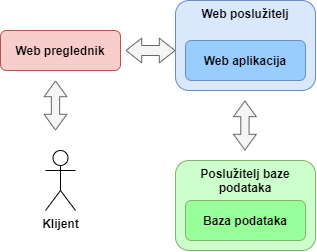
\includegraphics[scale=0.75]{slike/apstraktna-arh.PNG} %veličina slike u odnosu na originalnu datoteku i pozicija slike
	\centering
	\caption{Apstraktna arhitektura sustava}
	\label{fig:arh}
\end{figure}
\vspace{15pt}

\underline{Web preglednik} (eng. web browser) je program koji korisniku omogućuje pregled web-stranica i multimedijalnih sadržaja vezanih uz njih. Preglednik omogućuje komunikaciju između klijenta i poslužitelja. Dakle, korisnik će putem preglednika slati zahtjeve poslužitelju te će preglednik znati prikazati sadržaj koji poslužitelj vraća. \par
\vspace{10pt}
\underline{Web poslužitelj}  ima zadatak da pohranjuje, obrađuje i dostavlja klijentima web
stranice. Komunikacija između web poslužitelja i web klijenta (najčešće, web
pretraživača) odvija se korištenjem HTTP i drugih sličnih protokola (HTTPS,
HTTP/2 i različitih nadogradnji tih protokola). U komunikaciji putem HTTP-a, web
poslužitelj tipično sluša nadolazeće zahtjeve klijenata na portu 80. Web stranice koje
web poslužitelj isporučuje klijentu su HTML dokumenti, koji uključuju tekst, slike,
stilove, skripte i drugi sadržaj. \par
\vspace{10pt}
\underline{Web aplikacija} obrađuje korisnikove zahtjeve te ako je potrebno, pristupa bazi podataka i dohvaća/mijenja podatke. Nakon toga preko poslužitelja vraća korisniku odgovor u obliku HTML dokumenta koji se prikazuje u web pregledniku.\par
\vspace{10pt}
\underline{Baza podataka} pohranjuje podatke na sustavan način.  Računalni program korišten za upravljanje i ispitivanje baze podataka nazvan je sustav upravljanja bazom podataka (SUBP).\par

\vspace{15pt}
	
	Arhitektura i stil našeg sustava se može identificirati kao \textbf {višeslojni stil arhitekture}. Naime, naša arhitektura je uglavnom definirana činjenicom da koristimo \textbf{Spring Boot}. Obrazac koji se koristi u okviru radnog okvira Spring Boot je jedan od suvremenih primjera organizacije višeslojne arhitekture, a karakteriziraju ga dva principa:
	\begin{itemize}
		\item inverzija upravljanja (engl. inversion of control)
		\item ubacivanje ovisnosti (engl. dependency injection)
	\end{itemize}

	\underline{Inverzija upravljanja} funkcionira tako da korisnički napisani dijelovi (web) aplikacije
	dobiju upravljački tok i izvode se kada ih prozove neki generički radni okvir.  To je
	inverzno u odnosu na tradicionalno programiranje u kojem korisnički kôd poziva
	određene knjižnice kako bi se mogao izvršavati. U slučaju inverzije upravljanja, radni
	okvir za web aplikacije (u ovom slučaju, Spring Boot) poziva korisnički kod.
	
	\underline{Ubacivanje ovisnosti} je najčešći način kako u praksi funkcionira inverzija upravljanja. Korisnički kod prima kao argumente metoda određene objekte, koji se u ovoj terminologiji zovu uslugama (engl. service), a koji su specificirani od strane radnog
	okvira kako bi sustav uspješno radio. Tako radni okvir, koji se u ovoj terminologiji
	naziva ubacivač ili injektor (engl. injector) ubacuje ovisnost o svojem određenom
	ugrađenom objektu u korisnički kod i definira sučelje (engl. interface) putem kojeg
	korisnički kôd pristupa usluzi. 
	
	\vspace{15pt} 
	
	Naša arhitektura se tako sastoji od slojeva:
	
	\begin{itemize}
		\item \underline{sloj korisničke strane} – implementiran u JavaScriptu, koristeći knjižnicu \textbf{React} koja omogućuje prikaz korisničkog sučelja
		\item \underline{sloj nadglednika} (engl. controller) – povezuje korisničku stranu s poslužiteljskom stranom
		\item \underline{sloj usluge} (engl. service) – obavlja svu poslovnu logiku i potrebne izračune
		\item \underline{sloj domene} (engl. domain) – ima razrađeni model podataka domene
		\item \underline{sloj za pristup podatcima} (engl. data access object, kraće: DAO) – koji
		omogućuje spremanje i dohvat podataka iz određene baze podataka te
		razmjenu tih podataka sa slojem domene
		\item \underline{sloj baze podataka} – koji omogućuje stvarnu pohranu podataka u neku bazu,(u našem slučaju relacijsku bazu Postgre). 
	\end{itemize} 

\vspace{15pt} 
\begin{figure}[H]
	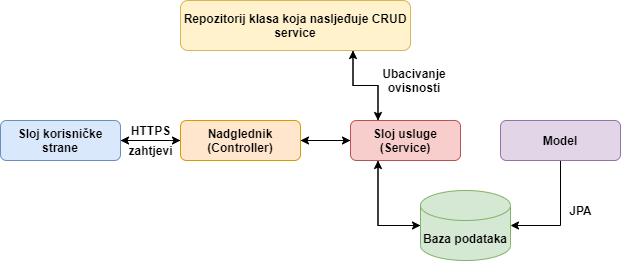
\includegraphics[scale=0.75]{slike/arhitektura.PNG} %veličina slike u odnosu na originalnu datoteku i pozicija slike
	\centering
	\caption{Spring Boot arhitektura}
	\label{fig:spring}
\end{figure}

Želimo li, radi lakšeg razumijevanja, našu arhitekturu usporediti sa stilom MVC (Model-View-Controller), možemo uočiti da se neki slojevi djelomično poklapaju. Primjerice sloj modela kod MVC-a
odgovarao bi sloju domene kod Spring Boota, sloj nadglednika kod MVC-a sloju
nadglednika kod Spring Boota, a sloj pogleda bio bi sloj korisničke strane. 


\vspace{15pt}
Kao što je navedeno, sloj korisničke strane (frontend) je implementiran u Java Scriptu koristeći knjižnicu React. \textbf{React} je besplatna biblioteka otvorenog koda za programski jezik JavaScript koja omogucava razvoj korisničkih sučelja SPA (eng. single-page application). SPA aplikacija je
tip web-aplikacije koja u interakciji s korisnikom dinamički mijenja dijelove stranice, za razliku od tradicionalnih web-aplikacija koje učitavaju cijele nove stranice s poslužitelja. One se pokreću u browseru i ne zahtijevaju ponovno učitavanje nakon korištenja.
React omogućava sastavljanje korisničkog sučelja pomoću elemenata koji se nazivaju komponente. Njih je mogucće iznova koristiti u aplikaciji proizvoljno veliki broj puta. Taj pristup pokazao se lakši za održavanje, proširivanje i višestruko korištenje.



	
		

		

				
		\section{Baza podataka}
			
			\textbf{\textit{dio 1. revizije}}\\
			
		\textit{Potrebno je opisati koju vrstu i implementaciju baze podataka ste odabrali, glavne komponente od kojih se sastoji i slično.}
		
			\subsection{Opis tablica}
			

				\textit{Svaku tablicu je potrebno opisati po zadanom predlošku. Lijevo se nalazi točno ime varijable u bazi podataka, u sredini se nalazi tip podataka, a desno se nalazi opis varijable. Svjetlozelenom bojom označite primarni ključ. Svjetlo plavom označite strani ključ}
				
				\begin{longtabu} to \textwidth {|X[6, l]|X[6, l]|X[20, l]|}
					
					\hline \multicolumn{3}{|c|}{\textbf{korisnik - ime tablice}}	 \\[3pt] \hline
					\endfirsthead
					
					\hline \multicolumn{3}{|c|}{\textbf{korisnik - ime tablice}}	 \\[3pt] \hline
					\endhead
					
					\hline 
					\endlastfoot
					
					\cellcolor{LightGreen}IDKorisnik & INT	&  	Lorem ipsum dolor sit amet, consectetur adipiscing elit, sed do eiusmod tempor incididunt ut labore et dolore magna aliqua. Ut enim ad minim veniam 	\\ \hline
					korisnickoIme	& VARCHAR &   	\\ \hline 
					email & VARCHAR &   \\ \hline 
					ime & VARCHAR	&  		\\ \hline 
					\cellcolor{LightBlue} primjer	& VARCHAR &   	\\ \hline 
					
					
				\end{longtabu}
			
			
			\subsection{Dijagram baze podataka}
				\textit{ U ovom potpoglavlju potrebno je umetnuti dijagram baze podataka. Primarni i strani ključevi moraju biti označeni, a tablice povezane. Bazu podataka je potrebno normalizirati. Podsjetite se kolegija "Baze podataka".}
			
			\eject
			
			
		\section{Dijagram razreda}
		
		\iffalse
			\textit{Potrebno je priložiti dijagram razreda s pripadajućim opisom. Zbog preglednosti je moguće dijagram razlomiti na više njih, ali moraju biti grupirani prema sličnim razinama apstrakcije i srodnim funkcionalnostima.}\\
			
			\textbf{\textit{dio 1. revizije}}\\
			
			\textit{Prilikom prve predaje projekta, potrebno je priložiti potpuno razrađen dijagram razreda vezan uz \textbf{generičku funkcionalnost} sustava. Ostale funkcionalnosti trebaju biti idejno razrađene u dijagramu sa sljedećim komponentama: nazivi razreda, nazivi metoda i vrste pristupa metodama (npr. javni, zaštićeni), nazivi atributa razreda, veze i odnosi između razreda.}\\
			
			\fi
			
			
			Na slikama su prikazani dijagrami razreda koji predstavljaju backend dio MVC arhitekture ostvarene korištenjem Java Spring Boota.
			
			\vspace{15pt} 
			\begin{figure}[H]
				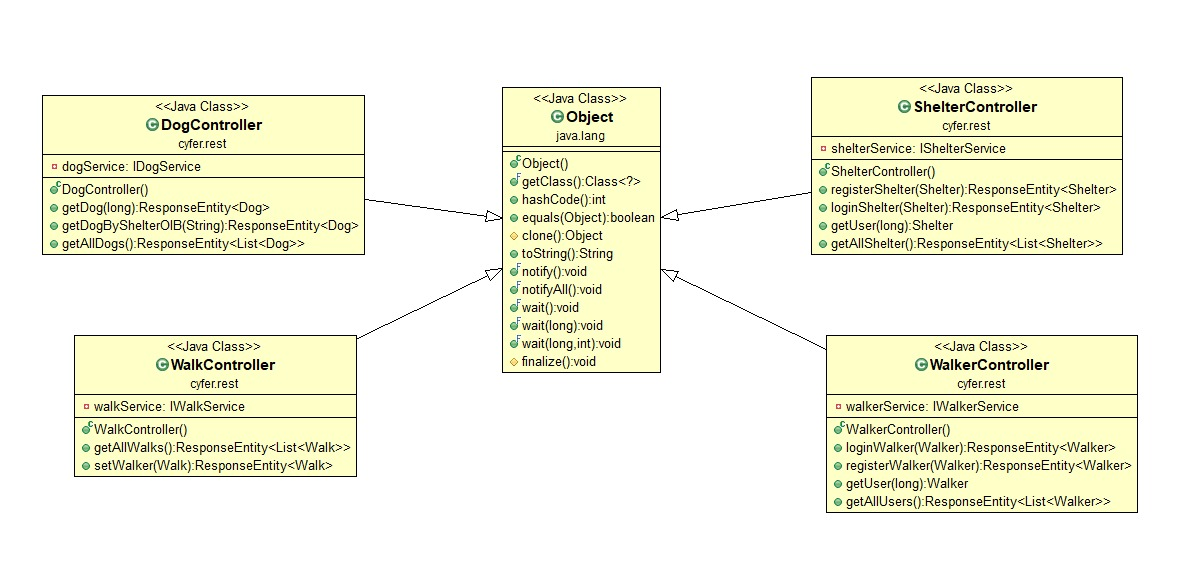
\includegraphics[scale=0.4]{dijagrami/controlleri.jpg} %veličina slike u odnosu na originalnu datoteku i pozicija slike
				\centering
				\caption{Razredi controlleri}
				\label{fig:controlleri}
			\end{figure}
			
			
			Razredi prikazani na slici 4.3 predstavljaju MVC Kontrolere čije metode mapiraju određene zahtjeve putem URI-a, te vraćaju JSON datoteke koje se potom obrađuju na određeni način. Također šalju i HTML statusni kod.
			Kontroleri su implementirani za četiri klase tipa Model: Dog, Walk, Shelter, Walker. Svaki razred ima konstruktor i metode koje mapiraju određene zahtjeve zadanim HTTP zahtjevom.
			
				\vspace{15pt} 
			\begin{figure}[H]
				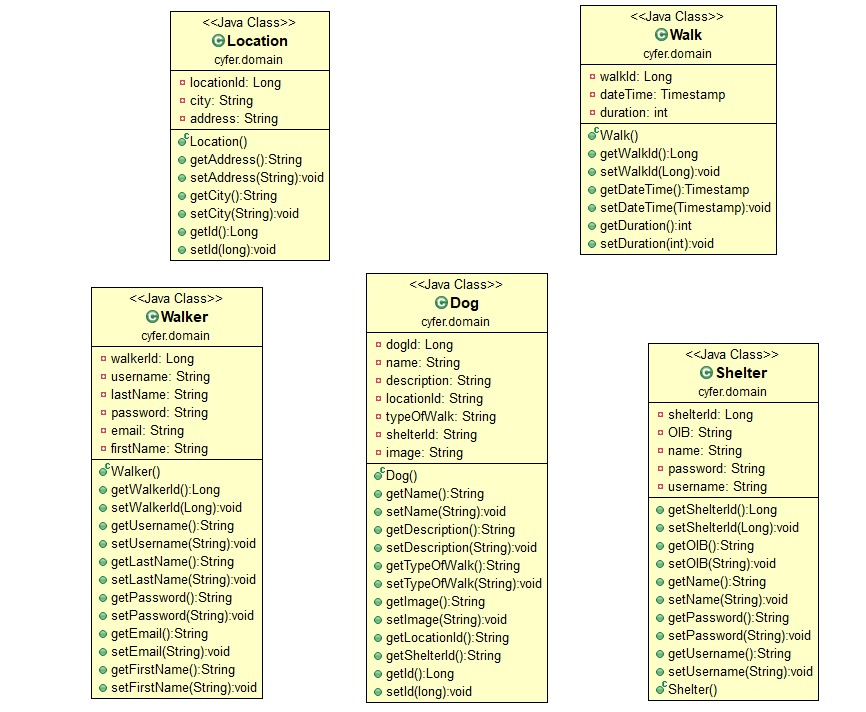
\includegraphics[scale=0.5]{dijagrami/modeli.jpg} %veličina slike u odnosu na originalnu datoteku i pozicija slike
				\centering
				\caption{Razredi modeli}
				\label{fig:modeli}
			\end{figure}
			
			
			Razredi prikazani na slici 4.4 predstavljaju MVC Modele koji odgovaraju entitetima u bazi podataka. Svaki razred sadrži svoj konstruktor, privatne članske varijable koje su mu svojstvene i koje odgovaraju atributima u bazi, kao i sve gettere i settere.
			Razred Dog predstavlja psa koji je pridruženoj određenoj udruzi (Shelter) i dostupan je za šetnje. Razred Walker predstavlja registriranog korisnika (šetača) koji može odabrati psa/pse za šetnju. Razred Shelter predstavlja registriranu udrugu koja ima svoj profil i pse dostupne za šetnju. Razred Walk predstavlja šetnju koja se dogodila s jednim šetačom i jednim ili više pasa. Razred Location predstavlja lokaciju (grad i adresa) na kojoj može biti smješten pas ili udruga.
			
			
			\iffalse
			\textbf{\textit{dio 2. revizije}}\\			
			
			\textit{Prilikom druge predaje projekta dijagram razreda i opisi moraju odgovarati stvarnom stanju implementacije}
			
			\fi
			
			\eject
		
		\section{Dijagram stanja}
			
			
			\textbf{\textit{dio 2. revizije}}\\
			
			\textit{Potrebno je priložiti dijagram stanja i opisati ga. Dovoljan je jedan dijagram stanja koji prikazuje \textbf{značajan dio funkcionalnosti} sustava. Na primjer, stanja korisničkog sučelja i tijek korištenja neke ključne funkcionalnosti jesu značajan dio sustava, a registracija i prijava nisu. }
			
			
			\eject 
		
		\section{Dijagram aktivnosti}
			
			\textbf{\textit{dio 2. revizije}}\\
			
			 \textit{Potrebno je priložiti dijagram aktivnosti s pripadajućim opisom. Dijagram aktivnosti treba prikazivati značajan dio sustava.}
			
			\eject
		\section{Dijagram komponenti}
		
			\textbf{\textit{dio 2. revizije}}\\
		
			 \textit{Potrebno je priložiti dijagram komponenti s pripadajućim opisom. Dijagram komponenti treba prikazivati strukturu cijele aplikacije.}